\documentclass[a4paper,11pt]{article} %, landscape report

\usepackage[T1]{fontenc}
\usepackage[utf8x]{inputenc}

%Selon les goûts: times palatino bookman newcent chancery helvet avant fourier kpfonts cmbright
%\usepackage{avant}

%\usepackage[hmargin=2cm,vmargin=2cm]{geometry}
%\usepackage{multicol}
%\setlength{\columnsep}{1cm}
\usepackage{ragged2e}% for \justifiy

\usepackage{graphicx}
\usepackage{xcolor}
\usepackage{multicol}\setlength{\columnsep}{1cm}

\usepackage{amsmath,amssymb,amsfonts,makeidx}
\usepackage{stmaryrd}% crochets «intervalles d'entiers»
%\newcommand{\B}{\mathbb{B}}
\usepackage{tikz}
\newcommand{\e}{\text{e}}

\usepackage{lscape}

\newcommand{\vesp}{\vspace*{0.2em}}
\newcommand{\VESP}{\vspace*{0.8em}}
\newcommand{\ttt}[1]{\texttt{#1}}
\newcommand{\file}[1]{\colorbox{blue!10}{\texttt{#1}}}
\newcommand{\code}[1]{\textcolor{blue}{\texttt{#1}}}
\newcommand{\rem}[1]{\colorbox{yellow}{\textbf{#1}}}
\newcommand{\REM}[1]{\colorbox{yellow}{\color{red}\textbf{#1}}}
\newcommand{\evid}[1]{\colorbox{blue!10}{\textbf{#1}}}

\usepackage{hyperref}
\hypersetup{colorlinks=true,
            linkcolor=violet,
            urlcolor=teal,
            citecolor=olive,
            }
\newcommand{\www}[2]{\href{#1}{\nolinkurl{#2}}}
%black, blue, brown, cyan, darkgray, gray, green, lightgray, lime, magenta, olive, orange, pink, purple, red, teal, violet, white, yellow
%\urlstyle{same}% Pas stylés \og URL

%\usepackage[nosort]{cite}

%\usepackage{minted}
%\usemintedstyle{%friendly, %colorful, %autumn
%    breaklines, fontfamily=courier,%helvetica,%tt,
%    bgcolor=gray!10,
%    %framesep=2mm,
%    %fontsize=\large,
%    %frame=lines,%single,
%    numbers=none,%left,
%    autogobble, mathescape, texcomments,
%    %stepnumber=2,
%    escapeinside=\%
%}
%% Inline
%\newcommand{\Py}[1]{\mintinline[bgcolor=gray!15]{python}{#1}}
%\newcommand{\BPy}[1]{\textbf{\Py{#1}}}
%\newcommand{\SerreCode}{\vspace*{-0.8em}}
\newcommand{\Py}[1]{\colorbox{gray!20}{\texttt{#1}}}

%\newcommand{\1}{\textcircled{\small 1}}
%\newcommand{\2}{\textcircled{\small 2}}
\setlength{\parskip}{0.2em}
%\setlength{\parindent}{0ex}

\usepackage[french]{babel} \frenchbsetup{StandardLists=true}
\usepackage[autolanguage]{numprint}
\DecimalMathComma

\AddThinSpaceBeforeFootnotes
\FrenchFootnotes

% =================================================================================================
\title{\textbf{Implémentation de la DP dans pytorch-dp\\{\small Exemple avec le MNIST}}}
\author{}
\date{}

\begin{document}%\setlength\parindent{5mm}
\maketitle
%%
\section{Ajout du bruit pour l'entraînement}
%%

%
\subsection{Organisation générale de l'exemple du MNIST}
%

Dans le fichier file{mnist.py},
\begin{itemize}
    \item
    La fonction principale \code{main()} commence par \textbf{parser les arguments} de la ligne de commande, notamment\\
        \ttt{--batch-size} (par défaut $64$),\\
        \ttt{--epochs} ($14$, nombre de répétitions des cycles complets),\\
        \ttt{-lr} ($1.0$, \emph{learning rate}),\\
        \ttt{--sigma} ($1.0$, futur écart-type $\sigma$ du bruit gaussien)\\
        \ttt{--max-per-sample-grad\_norm} ($1.0$, seuil du \emph{clipping}),\\
        \ttt{--delta} ($10^{-5}$, paramètre $\delta$ de la $(\varepsilon,\,\delta)$-DP)
    \item
    Puis (l. 234 \emph{numérotation dans \og ma\fg{} version commentée}) on crée les instances  \code{train\_loader} et \code{test\_loader} (en indiquant leur taille de \emph{batch} à chacun\footnote{Le \textbf{\emph{batch}} est l'ensemble des données utilisées avant la mise à jour des paramètres du modèle lors de l'entraînement, alors que l'\textbf{\emph{epoch}} correspond au parcours de l'ensemble des données d'entraînement. On parle respectivement de \emph{Stochastic~/ batch~/ mini-batch Gradient Descent} quand la taille du \emph{batch} vaut $1$~/ la taille du \emph{training set}~/ entre les deux. \url{https://machinelearningmastery.com/difference-between-a-batch-and-an-epoch/}}. de \ttt{torch.utils.data.Dataloader}. Les données seront téléchargées si besoin.
    \item
    Ensuite vient la phase d'entraînement (l. 278). On crée l'instance \code{model} de \ttt{SampleConvNet}, définie dans le même fichier comme sous-classe de  \ttt{pytorch.nn.Module}. Puis \code{optimizer}, de classe \ttt{torch.optim.SGD}, sans considération de DP à ce stade.
    \item
    La DP est alors implantée dans \code{model}:
    \begin{itemize}
        \item
            l. 293, on crée \code{privacy\_engine}, instance de \code{PrivacyEngine} avec en arguments\\
            \code{model}\\
            \code{train\_loader}\\
            \code{alphas} une liste des coefficients $\alpha$ (\emph{cf.} Rényi-DP) valant {\ttt{[1.1, 1.2, 1.3, ..., 10.9, 12, 13, ..., 63]}}\\
            \code{noise\_multiplier} ($\sigma$, passé en argument du script)\\
            \code{max\_grad\_norm} (seuil de \emph{clipping}, idem).
        \item
        L'appel (l. 304) à sa méthode \code{.attach(optimizer)} transforme sa phase d'entraînement en version DP ---~détaillé plus bas.
    \end{itemize}
    \item
    La fonction \code{train()}\footnote{Cette fonction fait également intervenir la DP, au niveau calcul du budget de confidentialité, on en parle plus loin.} définie dans le même fichier est appelée \ttt{epoch} fois, pour l'entraînement. Puis la valeur de retour de \code{test()}, fonction définie également dans ce fichier, est ajoutée à la liste \code{run\_results} dont la moyenne indiquera la justesse (\emph{accuracy}) du modèle...
\end{itemize}
%
\subsection{De la version standard à la DP}
%

La classe \code{PrivacyEngine} est définie dans le fichier \file{privacy\_engine.py}.
\begin{itemize}
    \item
    Les éléments locaux suivants sont importés:
        \begin{itemize}
        \item
        le module \ttt{privacy\_analysis as tf\_privacy}, repris du code TensorFLow Privacy de Google, gérant la RDP du mécanisme gaussien ---~détaillé plus bas.
        \item
        \ttt{PerSampleGradientClipper} du module \ttt{per\_sample\_gradient\_clip} qui prend en charge le \emph{clipping} des gradients, couche par couche.
        \item
        \ttt{DPModelInspector} du module \ttt{dp\_model\_inspector} pour vérifier que le modèle est compatible avec la transformation en version DP.
    \end{itemize}

    \item
    Le constructeur de \code{PrivacyEngine} reprend comme attributs les valeurs passées en paramètres, donc \code{module} pour qui recevra l'objet \code{model} instance de \ttt{SampleConvNet}. Il en crée aussi de nouveaux, dont:\\
         \code{sample\_rate}\ttt{ = dataloader.batch\_size / len(dataloader.dataset)},\\
         \code{validator}\ttt{ = DPModelInspector()},\\
         \code{clipper}\ttt{ = PerSampleGradientClipper(self.module, self.max\_grad\_norm)}

    \item
    La méthode \code{attach(optimizer)} permet de remplacer à chaud (\emph{monkey patching}) l'\emph{optimizer} d'origine par sa version DP, en redéclarant sa méthode \ttt{step}.

    \item
    La méthode \code{step()} de \ttt{PrivacyEngine} appelle son homonyme de \code{clipper} pour majorer les normes des gradients de chaque couche. Cette dernière est donc définie dans \file{per\_sample\_gradient\_clip.py} (l. 95):
    \begin{itemize}
        \item
        Appel de \ttt{autograd\_grad\_sample.compute\_grad\_sample(module)} qui crée un attribut \code{grad\_sample}, tenseur contenant les gradients calculés sur les données fournies d'entraînement. Les couches de type \ttt{Linear} et \ttt{Conv2d} sont prises en compte.\rem{Détailler  ?}
        \item
        Puis \ttt{clip\_per\_sample\_grad\_norm\_(module, max\_norm)} (fonction interne de \file{per\_sample\_gradient\_clip.py}) assure le \emph{clipping} des gradients, et enfin le calcul de leur moyennes  par batch\footnote{Elle utilise l'itérateur \ttt{torch.nn.Module.parameters()} pour traiter chacun des éléments du réseau neuronal.}, enregistrées dans l'attribut \code{grad}.
    \end{itemize}
    \item
    Ensuite, pour chaque élément du réseau, le \textbf{bruit gaussien} est ajouté\footnote{\emph{Idem}.}. Il est centré et d'écart-type  \ttt{noise\_multiplier * max\_grad\_norm} (soit $\sigma C$ en notation de l'algorithme 1 de l'article arXiv:1607.00133 \emph{Deep Learning with Differential Privacy}). Plus précisément, on crée un tenseur aléatoire \ttt{noise} de même \emph{shape} que celui qui représente le gradient associé à la couche traitée, puis on ajoute à ce dernier \ttt{noise} divisé par la taille du batch. En effet, la moyenne de chaque gradient a déjà été effectuée, on distribue donc dans la formule indiquée dans l'algorithme le facteur $\frac{1}{L}$ sur chacun des termes avant de les additionner. Les gradients bruités sont à nouveau stockés dans l'attribut \code{grad}.

\end{itemize}

Les \emph{shapes} des éléments \og paramètres\fg{} itérés permettent de comprendre leur nature quand on les met en parallèle avec l'architecture du réseau neuronal: [16, 1, 8, 8] (kernel de convolution pour $16$ couches en sortie, 1 niveau en entrée, en dimensions $8\times8$), puis [16] (ReLU sur chaque couche; rien concernant le \emph{max-pooling}), [32, 16, 4, 4] (convolution, idem), [32] (ReLU), puis [10, 288] (couche complètetement connectée, des $3\times3\times32$ valeurs ré-alignées vers les $10$ catégories en sortie).\\
\hspace*{-0.2\textwidth}
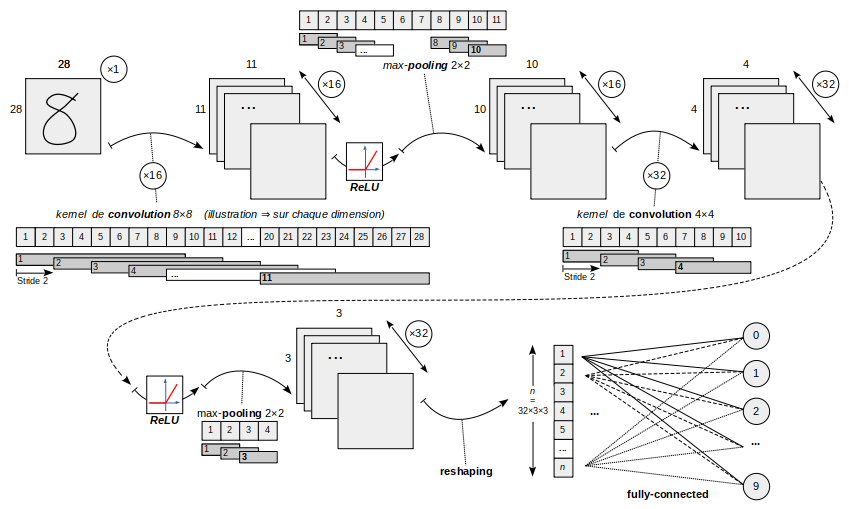
\includegraphics[width=1.4\textwidth]{cnn.png}

%%
\section{Optimisation du budget de DP}
%%
La fonction \code{train()} du fichier \file{mnist.py} qui affiche les performances appelle la méthode  \code{get\_privacy\_spent(targeted\_delta)} de \file{privacy\_analysis.py} qui renvoie les valeurs optimales de $\varepsilon$ et du $\alpha$ associé [en parcourant les points $(\alpha,\,\varepsilon)$ sur la \og courbe de budget\fg{} de confidentialité \emph{cf.} article \og Rényi-DP\fg{}, pour la liste des ordres $\alpha$ qu'on se donne].

Cette méthode utilise la fonction homonyme de \file{privacy\_analysis.py} à qui l'on passe la listes des $\alpha$ utilisables, le tenseur \code{rdp} [qui semble présenter les $\varepsilon$ courant de la $(\alpha,\,\varepsilon)$-RDP cumulée\rem{pas sûr ! vérifier...}] et le $\delta$ attendu. Elle ajoute (l. 209; terme à terme, pour chacune des données incluses dans ce tenseur) à \code{rdp}  la valeur $\frac{\ln(1/\delta)}{\alpha-1}$, conformément à la propriété 3 du IV. de l'article \og Rényi DP\fg{}: du $\varepsilon$ de la $(\alpha,\,\varepsilon)$-RDP on déduit à partir du $\delta$ attendu le $\varepsilon' = \varepsilon + \frac{\ln(1/\delta)}{\alpha-1}$ pour la $(\varepsilon',\,\delta)$-DP alors garantie.  Elle détermine enfin la valeur minimale de $\varepsilon$, avant de renvoyer le couple $(\varepsilon;\,\alpha)$ associé.
\\\rem{+ lien avec ce qui est affiché ; + comment cumuler /budget ?}


La valeur de \code{rdp} dans ce contexte de SGD est calculée par la méthode \ttt{get\_renyi\_divergence()} de \ttt{PrivacyEngine} qui utilise directement la fonction \code{compute\_rdp()} (l. 169) de \file{privacy\_analysis.py}. Celle-ci multiplie par le nombre d'étapes (\emph{de batches ?} \rem{à vérifier}) les valeurs renvoyées par la fonction \og locale\fg{} \ttt{\_compute\_rdp(q, sigma, alpha)} où \ttt{q} représente le taux d'échantillonnage.
\\\rem{Calculs à justifier (vérifier la sensibilité 1) Grossièrement :}
\begin{itemize}
    \item
    Cas q=1 / corollaire 3 VI de l'article \og RDP\fg{}
    \item
    Sinon, dans arXiv:1908.10530 "Rényi-DP of Sampled Gaussian Mecanism", conséquence en section 3 du théorème 4 et corollaire 7. pour justifier le $\varepsilon \leqslant \frac{\ln (A_\alpha)}{\alpha - 1}$ suffisant pour avoir la $(\varepsilon,\,\alpha)$-RDP.\\
    Puis pour le calcul de $A_\alpha$ soit entier soit en fraction, même article 3.3 page 11.
\end{itemize}





\end{document}